\clearpage
\newpage
\section{E field using electrical diagram}\label{sec:elDiagram}
The electric field in the LArIAT main drift volume can be determined knowing the voltage applied to the cathode, the voltage applied at the shield plane and the distance between t\
hem. We assume the distance between the cathode and the shield plane to be 470 mm and the voltage applied to the shield plane to be -298.75 V. The only quantity left to dermine is\
 then the voltage applied at the cathode. We can derive this latest quantity by using ohm's laws on the ciruit shown in fig \ref{fig:circuit}. We want to calculate the voltage at \
point B with respect to ground (point C). From ACNET readings, the volatge provided by the power supply is 23.5 kV and the glasmsman current reading is 0.0417 $\pm$ 0.015 mA (see \
figure \ref{fig:currentMeasurement}). LArIAT is equipped with two 40 $M\Omega$ filter pots in series, which correspond to an equivalent resistor of 80 $M\Omega$. Thus, the voltage\
 at the cathode is:

\begin{equation} V_{BC}=V_{PS} - I*R_{eq} = -23.5kV + 0.00417mA*80M\Omega = -23.17 kV, \label{eq:VBC}
\end{equation}
where I is the current and R$_{eq}$ is the equivalent resistor.
The electric field, drift voltage and drift time are then calculated to be

\begin{equation}E_{filed} = \frac{V_{BC} - V_{shield}}{\Delta x} = 486.54 \textit{ V/cm}
\end{equation}
\begin{equation}v_{drift} = \mu E_{field} = 1.5097 \textit{ mm/$\mu$s}
\end{equation}
\begin{equation}t_{drift} = \frac{\Delta x}{v_{drift}} = 311.316 \textit{ $\mu$s.}
\end{equation}

\begin{figure}[hp]
\centering
\begin{minipage}{0.45\textwidth}
\centering
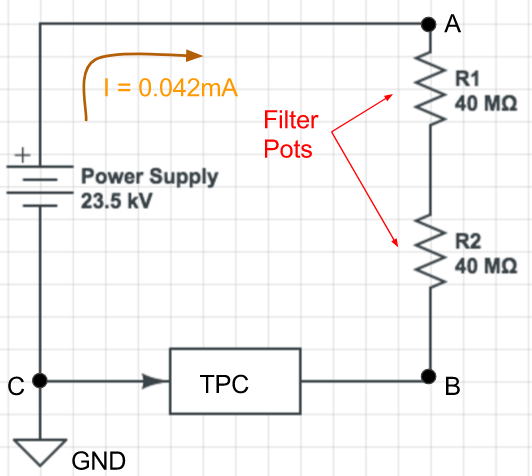
\includegraphics[width=3in]{images/CircuitLArIAT.png}
\caption{LArIAT HV simple schematics.}
\label{fig:circuit}
\end{minipage}\hfill
\begin{minipage}{0.45\textwidth}
\centering
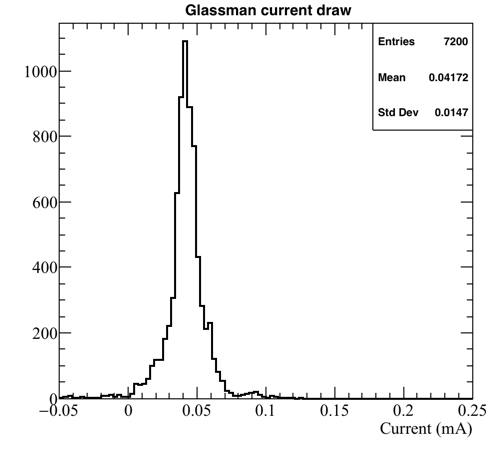
\includegraphics[width=3in]{images/glassman_current_20160525-30.png}
\caption{Current reading from the glassman between May 25th and May 30th 2016 (typical Run2 conditions).}
\label{fig:currentMeasurement}
\end{minipage}
\end{figure}
